%% CMDF table of dataset
The \acrfull{CMDf}\footnote{\url{http://compmusic.upf.edu/carnatic-rhythm-dataset}}\index{Carnatic music} is a rhythm annotated test corpus for many automatic rhythm analysis tasks in Carnatic Music~\cite{ajay:14:talaTrack}. The dataset consists of audio excerpts from the Carnatic research corpus, manually annotated time-aligned markers indicating the progression through the \gls{tala} cycle, and the associated \gls{tala} related metadata. 
\begin{table}[t]
\begin{center}
\tabcolsep=0.12cm
\begin{tabular}{@{}lrccrr@{}}
\toprule 
\Gls{tala} & \#Pieces & Total Duration & $\overline{\songlen}$ & \#Ann. & \#Sama\tabularnewline
 &  & hours (min) &  &  & \tabularnewline
\midrule 
\Gls{adi} & 50 & 4.21 (252.78) & 4m51s & 22793 & 2882\tabularnewline
\Gls{rupaka} & 50 & 4.45 (267.45) & 4m37s & 22668 & 7582\tabularnewline
\Gls{mishra chapu} & 48 & 5.70 (342.13) & 6m35s & 54309 & 7795\tabularnewline
\Gls{khanda chapu} & 28 & 2.24 (134.62) & 4m25s & 21382 & 4387\tabularnewline
\midrule 
Total & 176 & 16.61 (996.98) & 5m4s & 121602 & 22646\tabularnewline
\bottomrule 
\end{tabular}
\end{center}
\protect\caption[\acrshort{CMDf} dataset description]{\acrshort{CMDf} dataset showing the total duration and number of annotations. \#Sama shows the number of \gls{sama} annotations and \#Ann. shows the number of beat annotations (including \glspl{sama}). $\protect\overline{\protect\songlen}$ indicates the median piece length in the dataset (m and s indicate minutes and seconds, respectively)}
\label{tab:dataset:cmdf}
\end{table}
%% CMDF table of datastats
\begin{table}[t]
\centering
\begin{tabular}{@{}lccc@{}}
\toprule 
\Gls{tala} & $\overline{\isi} \pm \sigma_s$ & $\overline{\iai} \pm \sigma_o$ & $[{\isi}_{,\min} \, , \,  {\isi}_{,\max} ]$ \tabularnewline
\midrule 
\Gls{adi}  & 5.34 $\pm$ 0.723 & 0.167 $\pm$ 0.023 & $[$2.88, 7.07$]$\tabularnewline
\Gls{rupaka} & 2.13 $\pm$ 0.239 & 0.178 $\pm$ 0.020 & $[$1.21, 3.10$]$\tabularnewline
\Gls{mishra chapu} & 2.67 $\pm$ 0.358 & 0.191 $\pm$ 0.026 & $[$1.63, 3.65$]$\tabularnewline
\Gls{khanda chapu} & 1.85 $\pm$ 0.284 & 0.185 $\pm$ 0.028 & $[$0.91, 2.87$]$\tabularnewline
\bottomrule 
\end{tabular}
\protect\caption[\Gls{tala} cycle length indicators for \acrshort{CMDf} dataset]{\Gls{tala} cycle length indicators for \acrshort{CMDf} dataset. $\overline{\isi}$ and $\sigma_s$ indicate the mean and standard deviation of the median inter-\gls{sama} interval of the pieces, respectively. $\overline{\iai}$ and $\sigma_o$ indicate the mean and standard deviation of the median inter-\gls{akshara} interval of the pieces, respectively. $[{\isi}_{,\min} \, , \,  {\isi}_{,\max} ]$ indicate the minimum and maximum value of $\isi$ and hence the range of $\isi$ in the dataset. All values in the table are in seconds.}
\label{tab:datastat:cmdf}
\end{table}

\acrshort{CMDf} dataset is described in \tabref{tab:dataset:cmdf}, showing the four \glspl{tala} and the number of pieces for each \gls{tala}. The dataset has pieces in four popular \glspl{tala} that encompass a majority of current day Carnatic music performance. The pieces include a mix of vocal and instrumental recordings, recent and old recordings, and span a wide variety of forms. All pieces have a percussion accompaniment, predominantly mridangam. There are also several different pieces by the same artist (or release group), and multiple instances of the same composition rendered by different artists. Each piece is uniquely identified using the \gls{MBID} of the recording. The pieces are mp3 stereo recordings, and sampled at 44.1 kHz. The audio is also available as downmixed mono WAV files for experiments. The audio files are full length pieces or clips extracted from full length pieces. Of the 176 audio files, 120 contain full length pieces. 

There are several annotations that accompany each excerpt in the dataset. The primary annotations are audio synchronized time-stamps indicating the different metrical positions in the \gls{tala} cycle - the \gls{sama} (downbeat) and other beats shown with numerals in \figref{fig:taala:carnatic}. The annotations were created using Sonic Visualizer~\cite{cannam:10:sv} by tapping to music and manually correcting the taps. The annotations have been verified by a professional Carnatic musician. Each annotation has a time-stamp and an associated numeric label that indicates the position of the beat marker in the \gls{tala} cycle. In addition, for each excerpt, the \gls{tala} of the piece and \gls{edupu} (offset of the start of the piece, relative to the sama) are recorded. The possibly time varying tempo of a piece can be obtained using the beat and \gls{sama} annotations. 
%% CMD table of dataset
\begin{table}[t]
\centering
\begin{tabular}{@{}lrcrr@{}}
\toprule 
\Gls{tala} & \# Pieces & Total Duration & \# Ann. & \# Sama\tabularnewline
 &  & hours (min) &  & \tabularnewline
\midrule 
\Gls{adi} & 30 & 0.98 (58.87) & 5452 & 696\tabularnewline
\Gls{rupaka} & 30 & 1.00 (60.00) & 5148 & 1725\tabularnewline
\Gls{mishra chapu} & 30 & 1.00 (60.00) & 8992 & 1299\tabularnewline
\Gls{khanda chapu} & 28 & 0.93 (55.93) & 9133 & 1840\tabularnewline
\midrule 
Total & 118 & 3.91 (234.80) & 28725 & 5560\tabularnewline
\bottomrule 
\end{tabular}
\protect\caption[\acrshort{CMDs} dataset description]{\acrshort{CMDs} dataset showing the total duration and number of annotations. \#Sama shows the number of \gls{sama} annotations and \#Ann. shows the number of beat annotations (including \glspl{sama}).}
\label{tab:dataset:cmd}
\end{table}
%
%% CMD table of datastats
\begin{table}[t]
\centering
\begin{tabular}{@{}lccc@{}}
\toprule 
\Gls{tala} & $\overline{\isi} \pm \sigma_s$ & $\overline{\iai} \pm \sigma_o$ & $[{\isi}_{,\min} \, , \,  {\isi}_{,\max} ]$ \tabularnewline
\midrule 
\Gls{adi} & 5.32 $\pm$ 0.868 & 0.17 $\pm$ 0.027 & {[}2.88, 7.07{]}\tabularnewline
\Gls{rupaka} & 2.12 $\pm$ 0.225 & 0.18 $\pm$ 0.019 & {[}1.40, 3.10{]}\tabularnewline
\Gls{mishra chapu} & 2.81 $\pm$ 0.272  & 0.20 $\pm$ 0.019  & {[}2.03, 3.65{]}\tabularnewline
\Gls{khanda chapu} & 1.87 $\pm$ 0.290 & 0.19 $\pm$ 0.029 & {[}1.00, 2.84{]}\tabularnewline
\bottomrule 
\end{tabular}
\protect\caption[\Gls{tala} cycle length indicators for \acrshort{CMDs} dataset]{\Gls{tala} cycle length indicators for \acrshort{CMDs} dataset. $\overline{\isi}$ and $\sigma_s$ indicate the mean and standard deviation of the median inter-\gls{sama} interval of the pieces, respectively. $\overline{\iai}$ and $\sigma_o$ indicate the mean and standard deviation of the median inter-\gls{akshara} interval of the pieces, respectively. $[{\isi}_{,\min} \, , \,  {\isi}_{,\max}]$ indicate the minimum and maximum value of $\isi$ and hence the range of $\isi$ in the dataset. All values in the table are in seconds.}
\label{tab:datastat:cmd}
\end{table}

The total duration of audio in the dataset is over 16.6 hours, with 121062 time-aligned beat annotations. The median length of a piece is about 5 minutes in the dataset. \tabref{tab:datastat:cmdf} shows a basic statistical analysis of the \gls{tala} cycle length indicators in the dataset, which is useful to understand the tempo characteristics and the range of the metrical cycle lengths in the dataset. \Gls{adi} \gls{tala} is the longest \gls{tala} in the dataset and hence has the highest $\overline{\isi}$ among all the \glspl{tala}. Despite no notated tempo, we can see from the values of the median inter-\gls{akshara} interval, $\overline{\iai}$ and its standard deviation that the tempo in Carnatic music does not vary much across the \glspl{tala}. The range of $\overline{\isi}$ values show that a wide range of cycle durations that are present in Carnatic music pieces. The shortest cycle in the dataset is less than second long, while the longest cycle is over 7 seconds long. % spanning three tempo octaves. (, which means that we need more robust methods to handle tempo octave errors in tempo estimation.)The range of $\overline{\isi}$ values show that a wide range of tempi are present in Carnatic music pieces, often over two tempo octaves.
% Dataset stats: CMDf-ISI
\begin{figure}[t]
\centering
\subfloat[\Gls{adi}]{\label{fig:dstats:CMDf:ISI:adi}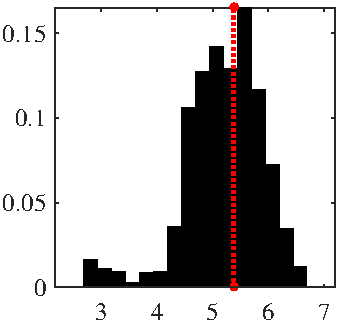
\includegraphics[scale=0.9]{dstats/CMDf-adi-ISI.pdf}} \hspace{0.5cm} 
\subfloat[\Gls{rupaka}]{\label{fig:dstats:CMDf:ISI:rupaka}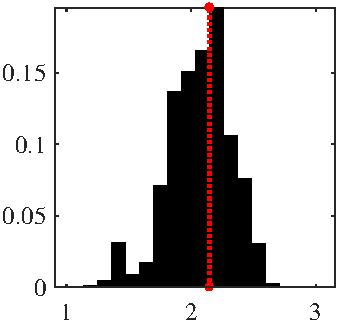
\includegraphics[scale=0.9]{dstats/CMDf-rupaka-ISI.pdf}} \\ 
\subfloat[\Gls{mishra chapu}]{\label{fig:dstats:CMDf:ISI:mishraChapu}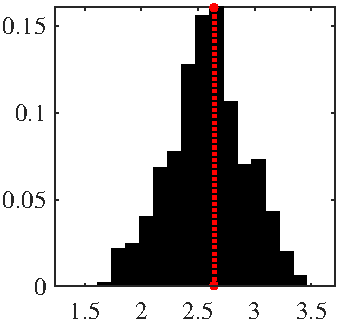
\includegraphics[scale=0.9]{dstats/CMDf-mishraChapu-ISI.pdf}} \hspace{0.5cm} 
\subfloat[\Gls{khanda chapu}]{\label{fig:dstats:CMDf:ISI:khandaChapu}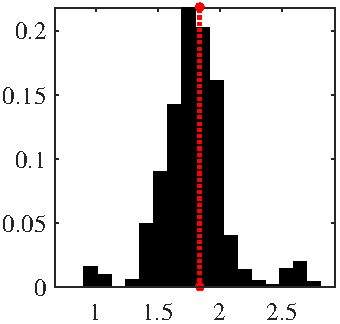
\includegraphics[scale=0.9]{dstats/CMDf-khandaChapu-ISI.pdf}} \\ 
\caption[Histogram of $\protect\isi$ in the \acrshort{CMDf} dataset]{A histogram of the inter-\gls{sama} interval $\protect\isi$ in the \acrshort{CMDf} dataset for each \gls{tala}. The ordinate is the fraction of the total count corresponding to the $\isi$ value shown in abscissa. The median $\isi$ for each \gls{tala} is shown as a red dotted line.}\label{fig:dstats:CMDf:ISI}
\end{figure}
% Dataset stats: CMDf-IAI
\begin{figure}[t]
\centering
\subfloat[\Gls{adi}]{\label{fig:dstats:CMDf:IAI:adi}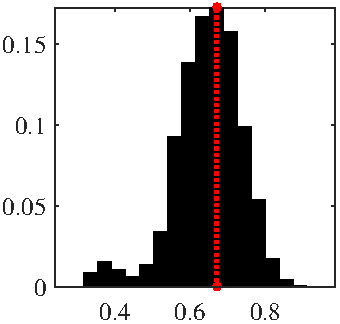
\includegraphics[scale=0.9]{dstats/CMDf-adi-IAI.pdf}} \hspace{0.5cm} 
\subfloat[\Gls{rupaka}]{\label{fig:dstats:CMDf:IAI:rupaka}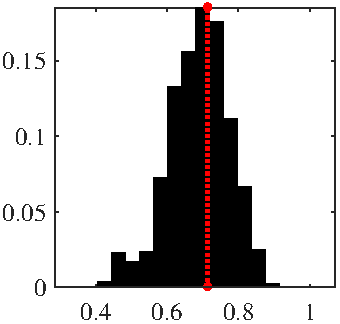
\includegraphics[scale=0.9]{dstats/CMDf-rupaka-IAI.pdf}} \\ 
\subfloat[\Gls{mishra chapu}]{\label{fig:dstats:CMDf:IAI:mishraChapu}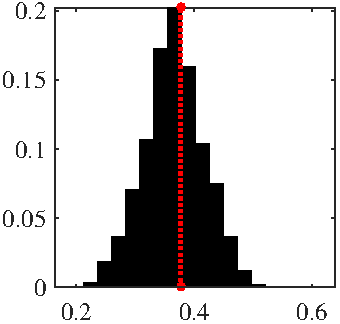
\includegraphics[scale=0.9]{dstats/CMDf-mishraChapu-IAI.pdf}} \hspace{0.5cm} 
\subfloat[\Gls{khanda chapu}]{\label{fig:dstats:CMDf:IAI:khandaChapu}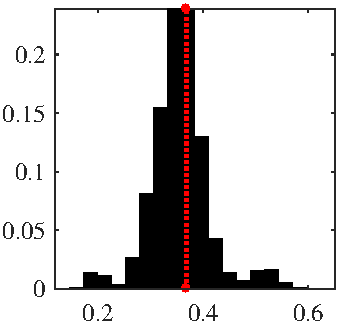
\includegraphics[scale=0.9]{dstats/CMDf-khandaChapu-IAI.pdf}} \\ 
\caption[Histogram of $\protect\ibi$ in the \acrshort{CMDf} dataset]{A histogram of the inter-beat interval $\protect\ibi$ in the \acrshort{CMDf} dataset for each \gls{tala}. The ordinate is the fraction of the total count corresponding to the $\ibi$ value shown in abscissa. The median $\ibi$ for each \gls{tala} is shown as a red dotted line.}\label{fig:dstats:CMDf:IAI}
\end{figure}
%
% Dataset stats: CMDf-ISInorm
\begin{figure}
%\captionsetup[subfigure]{labelformat=empty}
\begin{center}
\subfloat[\Gls{adi}]{\label{fig:dstats:CMDf:ISInorm:adi}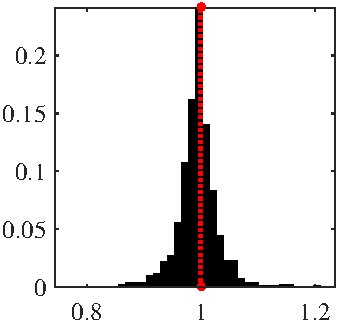
\includegraphics[scale=0.9]{dstats/CMDf-adi-ISInorm.pdf}} \hspace{0.5cm} 
\subfloat[\Gls{rupaka}]{\label{fig:dstats:CMDf:ISInorm:rupaka}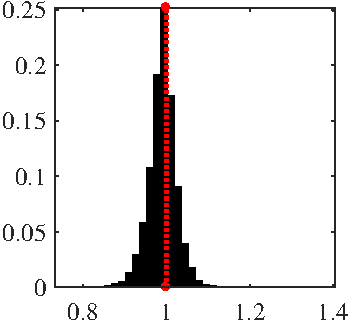
\includegraphics[scale=0.9]{dstats/CMDf-rupaka-ISInorm.pdf}} \\ 
\subfloat[\Gls{mishra chapu}]{\label{fig:dstats:CMDf:ISInorm:mishraChapu}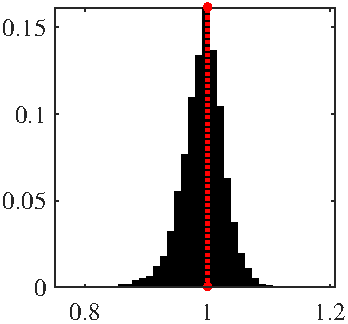
\includegraphics[scale=0.9]{dstats/CMDf-mishraChapu-ISInorm.pdf}} \hspace{0.5cm} 
\subfloat[\Gls{khanda chapu}]{\label{fig:dstats:CMDf:ISInorm:khandaChapu}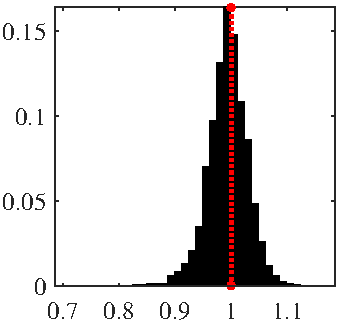
\includegraphics[scale=0.9]{dstats/CMDf-khandaChapu-ISInorm.pdf}} \\ 
\caption[Histogram of median normalized $\protect\isi$ in the \acrshort{CMDf} dataset]{A histogram of the median normalized inter-\gls{sama} interval $\protect\isi$ in the \acrshort{CMDf} dataset for each \gls{tala}. The ordinate is the fraction of the total count corresponding to the normalized $\isi$ value shown in abscissa.}\label{fig:dstats:CMDf:ISInorm}
\end{center}
\end{figure}
%
% Dataset stats: CMDf-IAInorm
\begin{figure}
%\captionsetup[subfigure]{labelformat=empty}
\begin{center}
\subfloat[\Gls{adi}]{\label{fig:dstats:CMDf:IAInorm:adi}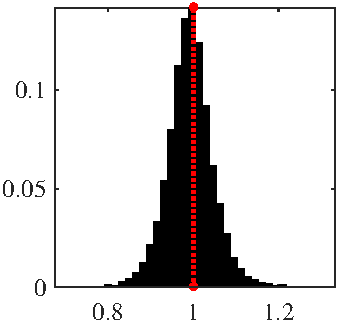
\includegraphics[scale=0.9]{dstats/CMDf-adi-IAInorm.pdf}} \hspace{0.5cm} 
\subfloat[\Gls{rupaka}]{\label{fig:dstats:CMDf:IAInorm:rupaka}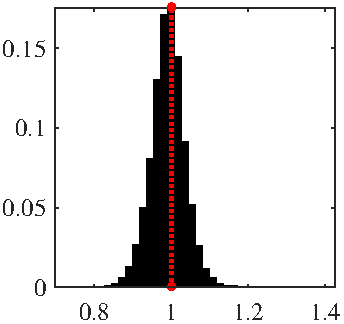
\includegraphics[scale=0.9]{dstats/CMDf-rupaka-IAInorm.pdf}} \\ 
\subfloat[\Gls{mishra chapu}]{\label{fig:dstats:CMDf:IAInorm:mishraChapu}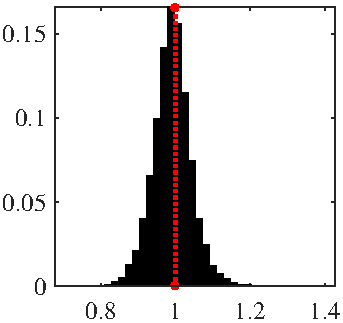
\includegraphics[scale=0.9]{dstats/CMDf-mishraChapu-IAInorm.pdf}} \hspace{0.5cm} 
\subfloat[\Gls{khanda chapu}]{\label{fig:dstats:CMDf:IAInorm:khandaChapu}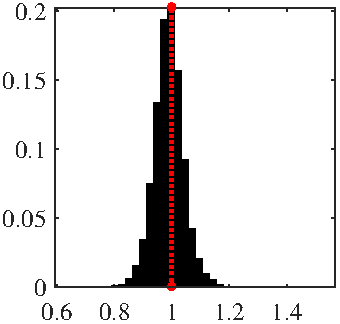
\includegraphics[scale=0.9]{dstats/CMDf-khandaChapu-IAInorm.pdf}} \\ 
\caption[Histogram of median normalized $\protect\ibi$ in the \acrshort{CMDf} dataset]{A histogram of the median normalized inter-beat interval $\protect\ibi$ in the \acrshort{CMDf} dataset for each \gls{tala}. The ordinate is the fraction of the total count corresponding to the normalized $\ibi$ value shown in abscissa.}\label{fig:dstats:CMDf:IAInorm}
\end{center}
\end{figure}

A representative subset of the \acrshort{CMDf} dataset is also compiled as the \acrshort{CMDs} dataset, with two minute excerpts of pieces in \acrshort{CMDf} (or the full piece if the piece is shorter than 2 minutes). These short excerpts additionally contain all the annotations of the full dataset, including time aligned \gls{sama} and beat annotations. The smaller \acrshort{CMDs} dataset will be useful for faster testing of approaches and algorithms. 

The \acrshort{CMDs} dataset is described in \tabref{tab:dataset:cmd}, showing the four \glspl{tala} and the number of pieces for each \gls{tala}. The total duration of audio in the dataset is about 4 hours, with 28725 time-aligned beat annotations. \tabref{tab:datastat:cmd} shows a basic statistical analysis of the \gls{tala} cycle length indicators in the \acrshort{CMDs} dataset, which are similar to the indicators of \acrshort{CMDf} dataset shown in \tabref{tab:datastat:cmdf}, showing that \acrshort{CMDs} dataset is a representative subset of \acrshort{CMDf} dataset. 

The tempo values are not notated in Carnatic music, and the pieces are not played to a metronome. Hence, in addition to the median values tabulated in \tabref{tab:datastat:cmdf} we present further analysis of the inter-\gls{sama} interval (\isi) and inter-beat interval (\ibi) for each \gls{tala} over the whole \acrshort{CMDf} dataset. A histogram of $\isi$ and $\ibi$ for each \gls{tala} is shown in \figref{fig:dstats:CMDf:ISI} and \figref{fig:dstats:CMDf:IAI} respectively. This shows the distribution of cycle lengths in the dataset over the whole range of $\isi$ for each \gls{tala}, around the median value. Despite the large range of $\isi$ values, the distribution in \figref{fig:dstats:CMDf:ISI} and \figref{fig:dstats:CMDf:IAI} show that the tempo often is limited to a small range of values. Though the musicians are free to choose any tempo, we empirically observe that they tend to choose a narrow range of tempo. 

To illustrate and measure the time varying tempo of music pieces in Carnatic music, we normalize all the $\isi$ and $\ibi$ values in a piece by the median value of the piece to obtain median normalized $\isi$ and $\ibi$ values, a histogram of which is shown for \acrshort{CMDf} dataset in \figref{fig:dstats:CMDf:ISInorm} and \figref{fig:dstats:CMDf:IAInorm}, respectively. These histograms are centered around 1 since they are normalized by the median, and the spread of these histograms around the value of 1 is a measure of deviation of tempo from the median value. From the figures, it is clear that the tempo is time varying but with less than about 20\% maximum deviation from the median tempo of the piece for all \glspl{tala}. 
% 
\subsubsection{Rhythm patterns in \acrshort{CMDf} and \acrshort{CMDs} datasets}
With a sizeable annotated corpus of Carnatic music, we can do corpora level analysis of patterns in rhythm\index{Rhythm pattern} and percussion. The idea is to showcase these patterns as a potential application of corpus level analysis, while showing their utility for meter tracking in \gls{MIR}, and for performance analysis and comparative analysis in musicology. 

The aim here is not to seek all musicological insights from data, but to illustrate the possibilities of a corpus level analysis data, and how such analysis tools can help aid and advance musicology. The \gls{MIR} applications of such datasets is the primary goal of the thesis and discussed in subsequent chapters. Hence, an example of corpus level musicological analysis is presented in this chapter, which amounts to a performance analysis of music in current practice from audio recordings. 

These analyses can corroborate several musicological inferences, and can provide additional insights into the differences between musicology, music theory and music practice. At the outset, it is necessary to note that the insights we discuss and conclusions we draw are limited by the available annotated dataset, and hence need further validation. It is however useful to focus on the methodology, which can aid musicologists and engineers to build systems that use these patterns for different analyses. 
\begin{figure}
\centering	
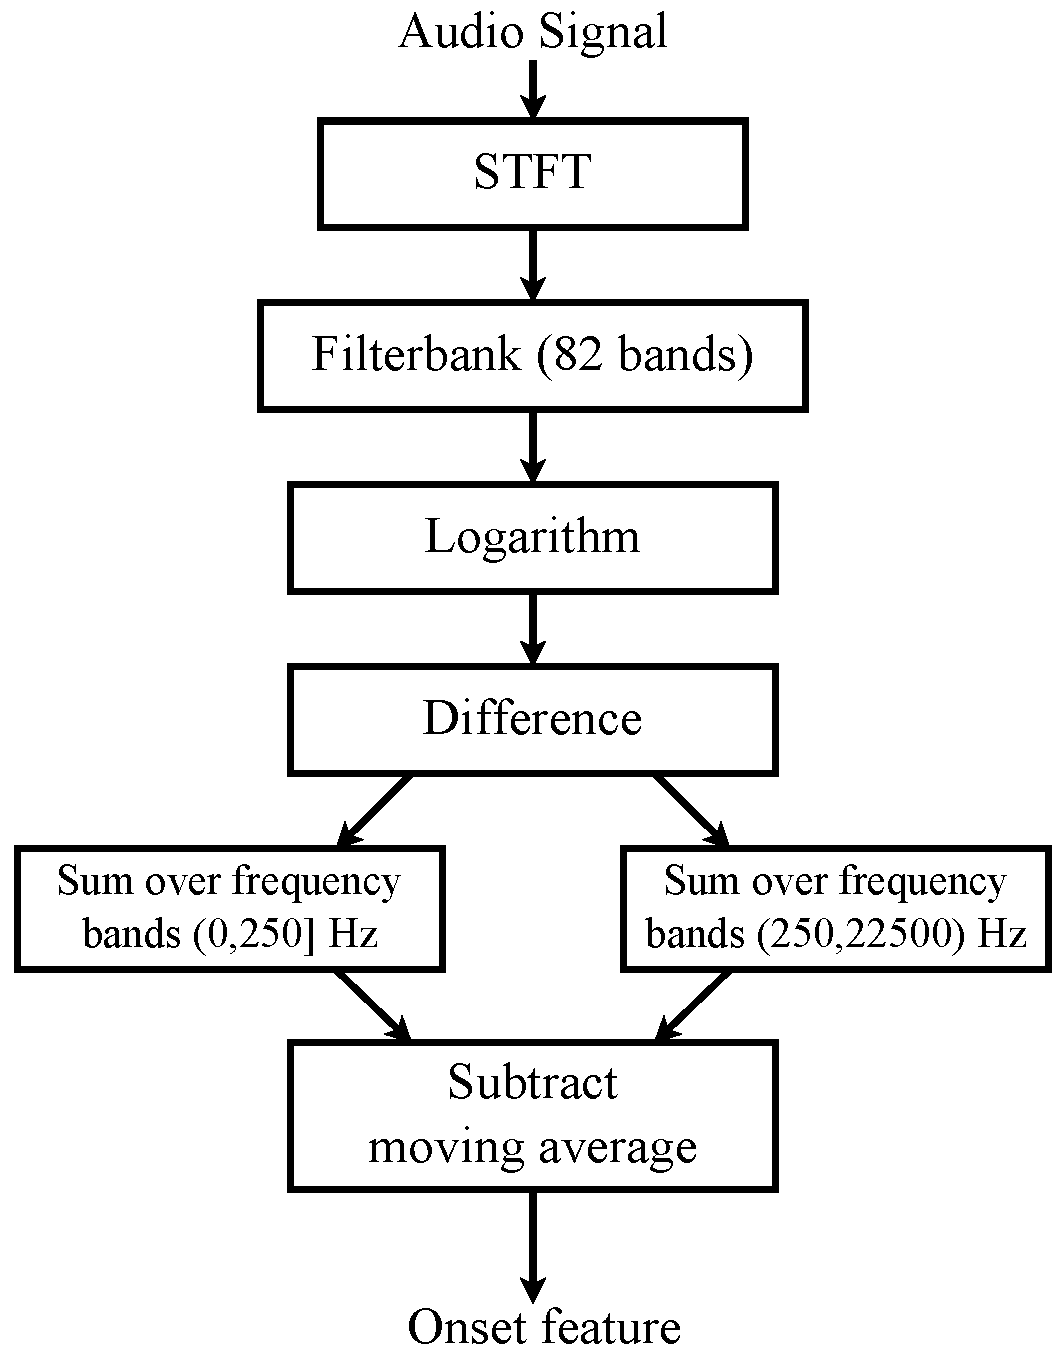
\includegraphics[scale=0.4]{blockDiags/obs-feat-computation.pdf}
	\caption[Computation of the spectral flux feature]{Computation of the spectral flux onset feature in two frequency bands, from \citeA{holzapfel:14:odd}.}
	\label{fig:obs:featcomp}
\end{figure}

The rhythm patterns are computed using a spectral flux\index{Spectral flux} feature (called LogFilt- SpecFlux as proposed by \citeA{bock:12:onseteval} and used further by \citeA{krebs:13:bpm}) that is used for detecting musical onsets in audio recordings. The \gls{STFT} of the audio signal with a window size of 46.4 ms (2047 samples of audio at a sampling rate of 44.1 kHz), DFT size of 2048 and hop size of 20 ms is computed from audio. The successive difference between frames of the logarithm of the filter bank energies in 82 different bands is then computed. Since the bass onsets have significant information about the rhythmic patterns, the features are computed in two frequency bands (Low: $\leq$ 250 Hz, High: $>$ 250 Hz) to additionally consider the bass onsets. The process of computing the spectral flux feature is outlined in \figref{fig:obs:featcomp}. 

Using beat and downbeat annotated training data, the audio features from all music pieces in a specific \gls{tala} are then grouped into cycle length sequences, and interpolated to equal lengths using a fine grid. A mean of all such cycle length sequence instances for a specific \gls{tala} is computed in both the frequency bands and used as a representative rhythmic pattern illustrated here. 

At the outset, it is necessary to note here that the patterns played in a \gls{tala} cycle are to be described using timing, energy and timbre descriptors. The rhythm patterns generated here using the spectral flux feature and can only explain timing and energy accents. A minor effect of timbre can be seen in these rhythm patterns, but are predominantly affected by the other two characteristics. These patterns are averaged over the whole dataset for a \gls{tala}, and hence cannot capture specific nuances of individual pieces, but only can give a broad perspective. The patterns here are indicative of the surface rhythm present in the audio recordings, and hence completely reflect the underlying canonical metrical structures. % List down other limitations of this approach. 

\figrefs{fig:tt:CMDf:adi}{fig:tt:CMD:khandaChapu}\ show the ensemble average of cycle length patterns over all the pieces in the dataset for each \gls{tala}, computed using the spectral flux feature in two different frequency bands as outlined above. In each figure, the bottom pane corresponds to the low frequency band ($\protect\obsLow$) and the top pane corresponds to the high frequency band ($\protect\obsHigh$). The abscissa is the beat number within the cycle (dotted lines), with 1 indicating the \gls{sama} (marked with a red line). The start of each \gls{anga} is indicated with beat numbers at the top of each pane (\gls{sama} shown as $\times$). The patterns in each figure pane is normalized so that maximum value is 1, to comment on relative onset strengths at different metrical positions of the cycle. 

The rhythm patterns are roughly indicative of the energies of mridangam strokes played in the cycle. In the figures, the bottom pane that shows the low frequency band has content from the left bass drum while the top pane has content predominantly from the right pitched drum (and additionally from the lead melody). Hence, for the purpose of this discussion, we use the terms left and right accents to refer to the accents in rhythm patterns shown on the bottom and top pane, respectively. The left and right accents provide interesting insights into the patterns played within a \gls{tala} cycle. In addition, these rhythm patterns help in meter tracking. 
% Tala pattern: CMDf-adi-all-lo230-superflux-mvavg-normZ, CMDf-adi-all-hi250-superflux-mvavg-normZ
\begin{figure}[t]
\captionsetup[subfigure]{labelformat=empty}
\centering
\subfloat[]{\label{fig:tt:CMDf:adi:hi}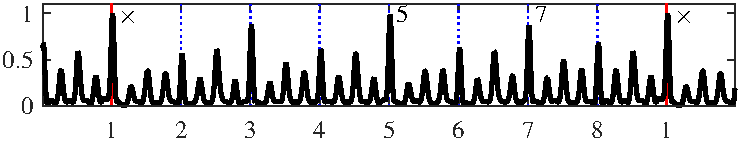
\includegraphics[width=\textwidth]{talaPatts/CMDf-adi-all-hi250-superflux-mvavg-normZ.pdf}} \\ \vspace{-1.35cm}
\subfloat[]{\label{fig:tt:CMDf:adi:lo}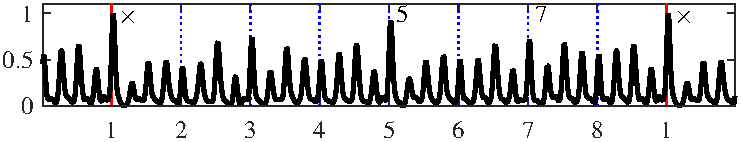
\includegraphics[width=\textwidth]{talaPatts/CMDf-adi-all-lo230-superflux-mvavg-normZ.pdf}}
\caption[Rhythm patterns in \gls{adi} \gls{tala} learned from \acrshort{CMDf} dataset]{Cycle length rhythmic patterns learned from \acrshort{CMDf} dataset for \gls{adi} \gls{tala}. In each of the following \protect\figrefs{fig:tt:CMDf:adi}{fig:tt:CMD:khandaChapu}, the patterns are computed from spectral flux feature and averaged over all the pieces in the dataset. The bottom/top pane corresponds to the low/high frequency bands, respectively. The abscissa is the beat number within the cycle (dotted lines), with 1 indicating the \gls{sama} (marked with a red line). The start of each \gls{anga} is indicated with beat numbers at the top of each pane (\gls{sama} shown as $\times$). The plot shows the cycle extended by a beat at the beginning and end to illustrate the cyclic nature of the \gls{tala}.}\label{fig:tt:CMDf:adi} %CMDf-adi-all-hi250-superflux-mvavg-normZ,CMDf-adi-all-lo230-superflux-mvavg-normZ
\end{figure}
%
% Tala pattern: CMD-adi-all-lo230-superflux-mvavg-normZ, CMD-adi-all-hi250-superflux-mvavg-normZ
\begin{figure}
\captionsetup[subfigure]{labelformat=empty}
\centering
\subfloat[]{\label{fig:tt:CMD:adi:hi}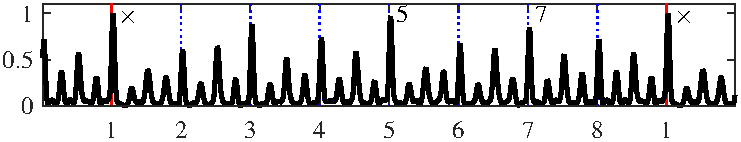
\includegraphics[width=\textwidth]{talaPatts/CMD-adi-all-hi250-superflux-mvavg-normZ.pdf}} \\ \vspace{-1.35cm}
\subfloat[]{\label{fig:tt:CMD:adi:lo}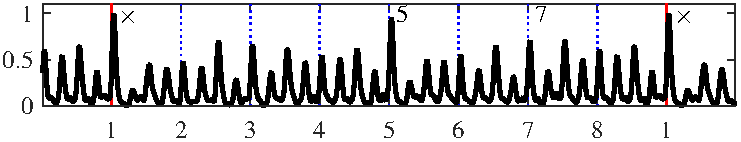
\includegraphics[width=\textwidth]{talaPatts/CMD-adi-all-lo230-superflux-mvavg-normZ.pdf}}
\caption[Rhythm patterns in \gls{adi} \gls{tala} learned from \acrshort{CMDs} dataset]{Cycle length rhythmic patterns learned from \acrshort{CMDs} dataset for \gls{adi} \gls{tala}.}\label{fig:tt:CMD:adi}
\end{figure}

We list down and discuss some salient qualitative observations from figures for each \gls{tala}, for both \acrshort{CMDf} dataset and its subset \acrshort{CMDs}. The \figrefs{fig:tt:CMDf:adi}{fig:tt:CMD:khandaChapu}\ show the cycle length rhythm patterns for all \glspl{tala} for both \acrshort{CMDf} and \acrshort{CMDs} datasets. For each \gls{tala}, we plot the rhythm patterns together to compare patterns across the short excerpts in \acrshort{CMDs} dataset and full length pieces in \acrshort{CMDf} dataset. 

Overall, we see stronger accents on the \glspl{akshara}, with \gls{sama} having the strongest accent in most cases. We can clearly see the accents organized in three different strengths, reflecting the metrical levels of the \gls{anga}, the beat and the \gls{akshara}. The two \gls{akshara} long beats in \gls{mishra chapu} and \gls{khanda chapu} \glspl{tala}, and the four \gls{akshara} long beats in \gls{adi} and \gls{rupaka} \glspl{tala} can be additionally seen. The patterns and \glspl{theka} played in Carnatic music are quite diverse, and no obvious representative \gls{tala} pattern can be inferred, apart from the varied accents at three metrical levels. 
% Tala pattern: CMDf-rupaka-all-lo230-superflux-mvavg-normZ, CMDf-rupaka-all-hi250-superflux-mvavg-normZ
\begin{figure}[t]
\captionsetup[subfigure]{labelformat=empty}
\centering
\subfloat[]{\label{fig:tt:CMDf:rupaka:hi}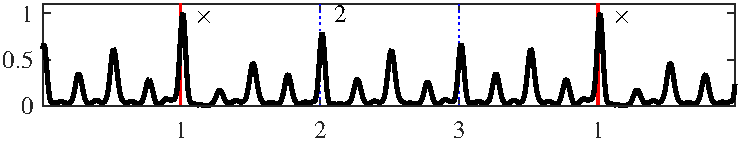
\includegraphics[width=\textwidth]{talaPatts/CMDf-rupaka-all-hi250-superflux-mvavg-normZ.pdf}} \\ \vspace{-1.35cm}
\subfloat[]{\label{fig:tt:CMDf:rupaka:lo}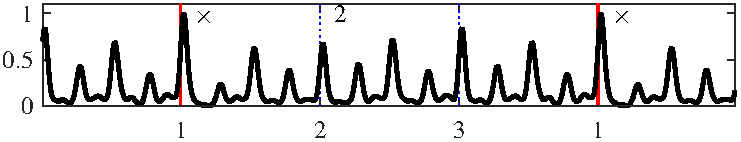
\includegraphics[width=\textwidth]{talaPatts/CMDf-rupaka-all-lo230-superflux-mvavg-normZ.pdf}}
\caption[Rhythm patterns in \gls{rupaka} \gls{tala} learned from \acrshort{CMDf} dataset]{Cycle length rhythmic patterns learned from \acrshort{CMDf} dataset for \gls{rupaka} \gls{tala}.}\label{fig:tt:CMDf:rupaka}
\end{figure}
%
% Tala pattern: CMD-rupaka-all-lo230-superflux-mvavg-normZ, CMD-rupaka-all-hi250-superflux-mvavg-normZ
\begin{figure}[t]
\captionsetup[subfigure]{labelformat=empty}
\centering
\subfloat[]{\label{fig:tt:CMD:rupaka:hi}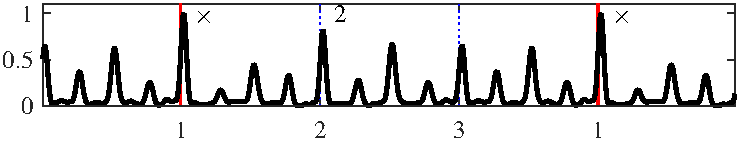
\includegraphics[width=\textwidth]{talaPatts/CMD-rupaka-all-hi250-superflux-mvavg-normZ.pdf}} \\ \vspace{-1.35cm}
\subfloat[]{\label{fig:tt:CMD:rupaka:lo}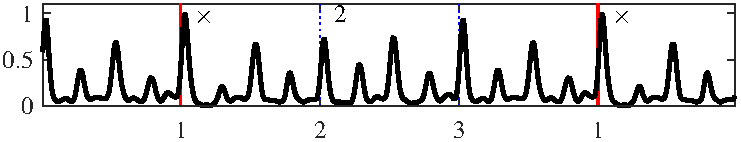
\includegraphics[width=\textwidth]{talaPatts/CMD-rupaka-all-lo230-superflux-mvavg-normZ.pdf}}
\caption[Rhythm patterns in \gls{rupaka} \gls{tala} learned from \acrshort{CMDs} dataset]{Cycle length rhythmic patterns learned from \acrshort{CMDs} dataset for \gls{rupaka} \gls{tala}.}\label{fig:tt:CMD:rupaka}
\end{figure}
%

The patterns illustrated here are average patterns that occur and do not tell us much about the various individual patterns that might occur in specific points in particular recordings. The \glspl{tala} are metrical structures that allow many different patterns to be played, and not a specific rhythm. It is further seen that the first \gls{akshara} after \gls{sama} has softer accents. Fewer strokes are played after the \gls{sama}, to emphasize that the \gls{sama} has just passed and a new cycle has begun. It might also perhaps indicate some form of recovery time after the intense stroke-playing towards the end of the cycle. 

The rhythm patterns computed using \acrshort{CMDs} dataset are very similar to those computed using \acrshort{CMDf} dataset, showing that \acrshort{CMDs} is a good representative subset of the larger \acrshort{CMDf}. Additionally, all the observations we make with patterns from \acrshort{CMDf} extend to \acrshort{CMDs}. We now discuss several \gls{tala} specific observations. 

The \figrefs{fig:tt:CMDf:adi}{fig:tt:CMD:adi}\ show the rhythm patterns for \gls{adi} \gls{tala}. We see that a three level hierarchy of \gls{anga}, beats and \glspl{akshara} is well demarcated. The \gls{akshara} at half cycle (beat 5) has an accent as strong as the \gls{sama}. The odd beats (marked 1, 3, 5, 7) have stronger right accents. The left accents are distributed through the cycle, with strong accents at half cycle.  
%
% Tala pattern: CMDf-mishraChapu-all-lo230-superflux-mvavg-normZ, CMDf-mishraChapu-all-hi250-superflux-mvavg-normZ
\begin{figure}[t]
\captionsetup[subfigure]{labelformat=empty}
\centering
\subfloat[]{\label{fig:tt:CMDf:mishraChapu:hi}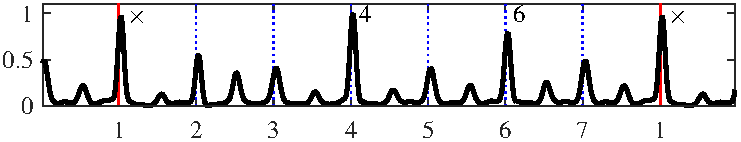
\includegraphics[width=\textwidth]{talaPatts/CMDf-mishraChapu-all-hi250-superflux-mvavg-normZ.pdf}} \\ \vspace{-1.35cm}
\subfloat[]{\label{fig:tt:CMDf:mishraChapu:lo}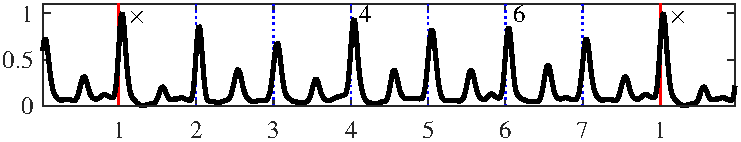
\includegraphics[width=\textwidth]{talaPatts/CMDf-mishraChapu-all-lo230-superflux-mvavg-normZ.pdf}}
\caption[Rhythm patterns in \gls{mishra chapu} \gls{tala} learned from \acrshort{CMDf} dataset]{Cycle length rhythmic patterns learned from \acrshort{CMDf} dataset for \gls{mishra chapu} \gls{tala}.}\label{fig:tt:CMDf:mishraChapu}
\end{figure}
%
%
% Tala pattern: CMD-mishraChapu-all-lo230-superflux-mvavg-normZ, CMD-mishraChapu-all-hi250-superflux-mvavg-normZ
\begin{figure}[t]
\captionsetup[subfigure]{labelformat=empty}
\centering
\subfloat[]{\label{fig:tt:CMD:mishraChapu:hi}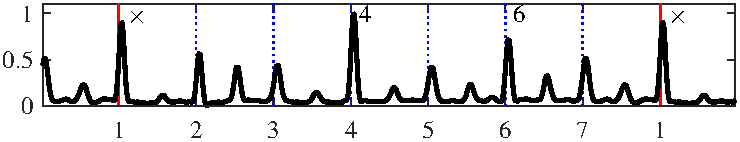
\includegraphics[width=\textwidth]{talaPatts/CMD-mishraChapu-all-hi250-superflux-mvavg-normZ.pdf}} \\ \vspace{-1.35cm}
\subfloat[]{\label{fig:tt:CMD:mishraChapu:lo}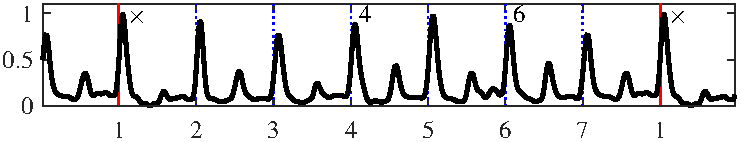
\includegraphics[width=\textwidth]{talaPatts/CMD-mishraChapu-all-lo230-superflux-mvavg-normZ.pdf}}
\caption[Rhythm patterns in \gls{mishra chapu} \gls{tala} learned from \acrshort{CMDs} dataset]{Cycle length rhythmic patterns learned from \acrshort{CMDs} dataset for \gls{mishra chapu} \gls{tala}.}\label{fig:tt:CMD:mishraChapu}
\end{figure}
%

The \figrefs{fig:tt:CMDf:rupaka}{fig:tt:CMD:rupaka}\ show the rhythm patterns for \gls{rupaka} \gls{tala}. Apart from the three level hierarachy of accents that is quite apparent, the half beat accent between the beats 2 and 3 are strong - indicating the often played 6+6 \gls{akshara} grouping structure of \gls{rupaka}, with a ternary meter.

The \figrefs{fig:tt:CMDf:mishraChapu}{fig:tt:CMD:mishraChapu}\ show the rhythm patterns for \gls{mishra chapu} \gls{tala}. We see that the \gls{anga} boundaries have strong left and right accents showing their use as anchor points to indicate the progression through the cycle. Though defined with a 3+2+2 \gls{akshara} grouping structure, a 1+2+2+2 structure is often seen in \gls{mishra chapu} \gls{tala}, which can be observed here, based on the strong left accent on beat 2. A additional strong left accent on beat 5 shows that it is also used as an anchor. 
%
% Tala pattern: CMDf-khandaChapu-all-lo230-superflux-mvavg-normZ, CMDf-khandaChapu-all-hi250-superflux-mvavg-normZ
\begin{figure}[t]
\captionsetup[subfigure]{labelformat=empty}
\centering
\subfloat[]{\label{fig:tt:CMDf:khandaChapu:hi}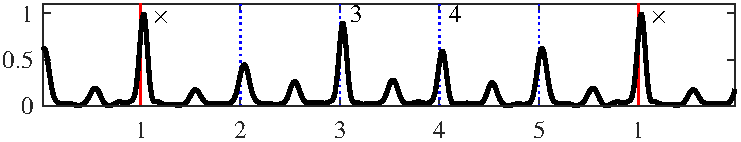
\includegraphics[width=\textwidth]{talaPatts/CMDf-khandaChapu-all-hi250-superflux-mvavg-normZ.pdf}} \\ \vspace{-1.35cm}
\subfloat[]{\label{fig:tt:CMDf:khandaChapu:lo}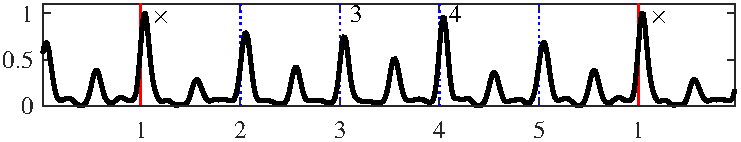
\includegraphics[width=\textwidth]{talaPatts/CMDf-khandaChapu-all-lo230-superflux-mvavg-normZ.pdf}}
\caption[Rhythm patterns in \gls{khanda chapu} \gls{tala} learned from \acrshort{CMDf} dataset]{Cycle length rhythmic patterns learned from \acrshort{CMDf} dataset for \gls{khanda chapu} \gls{tala}.}\label{fig:tt:CMDf:khandaChapu}
\end{figure}
%
%
% Tala pattern: CMD-khandaChapu-all-lo230-superflux-mvavg-normZ, CMD-khandaChapu-all-hi250-superflux-mvavg-normZ
\begin{figure}[t]
\captionsetup[subfigure]{labelformat=empty}
\centering
\subfloat[]{\label{fig:tt:CMD:khandaChapu:hi}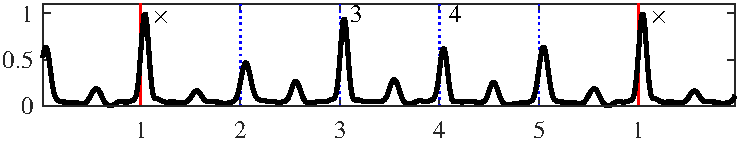
\includegraphics[width=\textwidth]{talaPatts/CMD-khandaChapu-all-hi250-superflux-mvavg-normZ.pdf}} \\ \vspace{-1.35cm}
\subfloat[]{\label{fig:tt:CMD:khandaChapu:lo}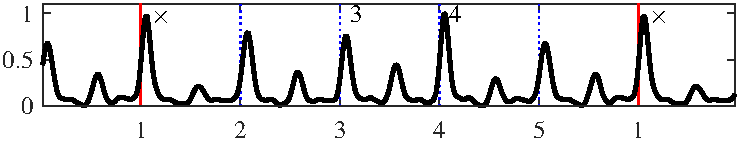
\includegraphics[width=\textwidth]{talaPatts/CMD-khandaChapu-all-lo230-superflux-mvavg-normZ.pdf}}
\caption[Rhythm patterns in \gls{khanda chapu} \gls{tala} learned from \acrshort{CMDs} dataset]{Cycle length rhythmic patterns learned from \acrshort{CMDs} dataset for \gls{khanda chapu} \gls{tala}.}\label{fig:tt:CMD:khandaChapu}
\end{figure}

The rhythm patterns of \gls{khanda chapu} \gls{tala} shown in \figrefs{fig:tt:CMDf:khandaChapu}{fig:tt:CMD:khandaChapu}\ have a strong left accent on beat 4, which is used an anchor within the cycle. A stronger right accent on beat 3 shows the progression through the unequal \glspl{anga}. The 2+1+2 \gls{akshara} grouping structure of \gls{khanda chapu} is often played out as 3+2 or 2+3, showing strong accents on beats 3 and 4. 

These are some observations from rhythm patterns that have interesting musicological significance. A professional Carnatic musician has informally validated these observations, but they still have to be formally studied in depth to make valid musicological conclusions. 
% An example of a corpus study with the dataset is an analysis of rhythmic patterns that occur in the dataset to see what musicological inferences can be made out of the analysis. We wish to independently verify 
% Statistical analysis of patterns in the dataset and what musicological inferences it can give out. 
%
%
%
% The bottom/top pane corresponds to the low/high frequency bands, respectively. The abscissa is the beat number within the cycle (dotted lines), with 1 indicating the \gls{sama} (marked with a red line). The start of each \gls{anga} is indicated with beat numbers at the top of each pane (\gls{sama} shown as $\times$).
\subsubsection{Applications of the Carnatic rhythm dataset}
The \acrshort{CMDf} dataset and its subset \acrshort{CMDs} dataset are intended to be test corpora for several automatic rhythm analysis tasks in Carnatic music. Possible tasks include \gls{sama} and beat tracking, tempo estimation and tracking, \gls{tala} recognition, rhythm based segmentation of musical audio, structural segmentation, audio to score/lyrics alignment, and rhythmic pattern analysis. In this thesis, these two datasets are primarily used for rhythmic pattern analysis and meter inference/tracking. Most of the research results are presented for \acrshort{CMDs} with some experiments extended to the full \acrshort{CMDf} dataset to verify their applicability to larger datasets.%\cite{ajay:14:rhythmJNMR, ajay:14:talaTrack} 
%
%
% Present stats about the dataset, then about distribution of ISI and IAI. Statistical analysis of patterns in the dataset and what musicological inferences it can give out. 
%
%% Dataset stats: CMD-IAI
\begin{figure}[ht]
%\captionsetup[subfigure]{labelformat=empty}
\begin{center}
\subfloat[\Gls{adi}]{\label{fig:dstats:CMD:IAI:adi}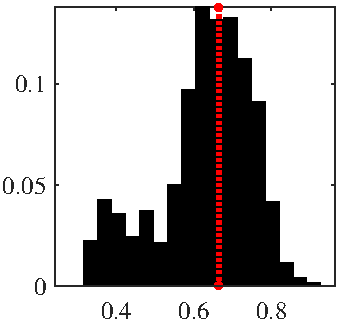
\includegraphics[scale=1]{dstats/CMD-adi-IAI.pdf}} \hspace{0.5cm} 
\subfloat[\Gls{rupaka}]{\label{fig:dstats:CMD:IAI:rupaka}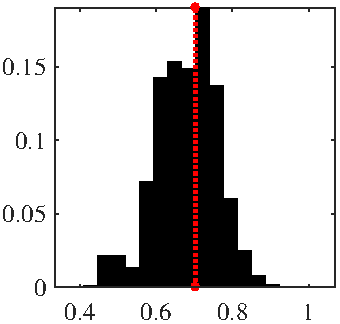
\includegraphics[scale=1]{dstats/CMD-rupaka-IAI.pdf}} \\ 
\subfloat[\Gls{mishra chapu}]{\label{fig:dstats:CMD:IAI:mishraChapu}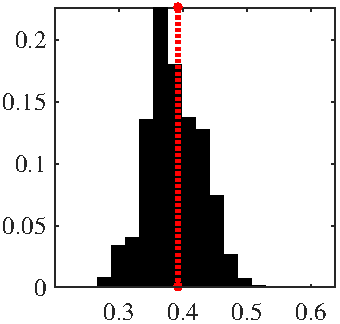
\includegraphics[scale=1]{dstats/CMD-mishraChapu-IAI.pdf}} \hspace{0.5cm} 
\subfloat[\Gls{khanda chapu}]{\label{fig:dstats:CMD:IAI:khandaChapu}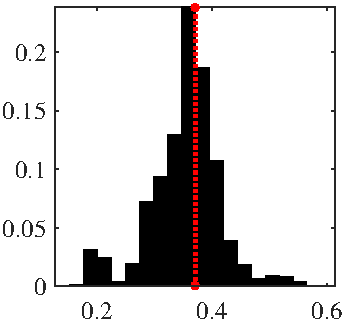
\includegraphics[scale=1]{dstats/CMD-khandaChapu-IAI.pdf}} \\ 
\caption[CMD-IAI]{CMD-IAI}\label{fig:dstats:CMD:IAI}
\end{center}
\end{figure}
%
%
% Dataset stats: CMD-IAInorm
\begin{figure}[ht]
%\captionsetup[subfigure]{labelformat=empty}
\begin{center}
\subfloat[\Gls{adi}]{\label{fig:dstats:CMD:IAInorm:adi}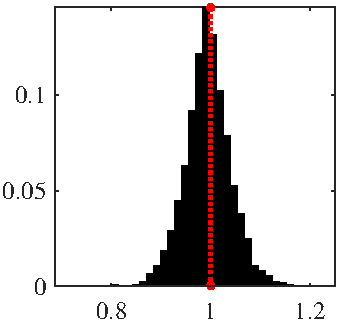
\includegraphics[scale=1]{dstats/CMD-adi-IAInorm.pdf}} \hspace{0.5cm} 
\subfloat[\Gls{rupaka}]{\label{fig:dstats:CMD:IAInorm:rupaka}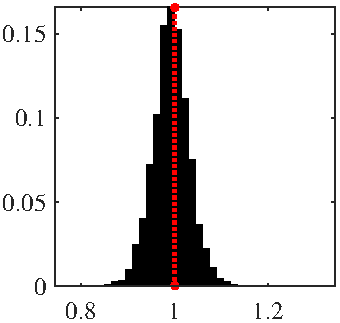
\includegraphics[scale=1]{dstats/CMD-rupaka-IAInorm.pdf}} \\ 
\subfloat[\Gls{mishra chapu}]{\label{fig:dstats:CMD:IAInorm:mishraChapu}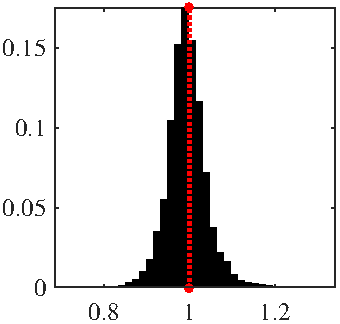
\includegraphics[scale=1]{dstats/CMD-mishraChapu-IAInorm.pdf}} \hspace{0.5cm} 
\subfloat[\Gls{khanda chapu}]{\label{fig:dstats:CMD:IAInorm:khandaChapu}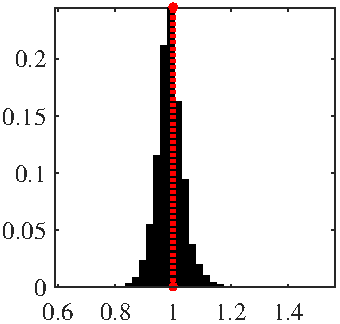
\includegraphics[scale=1]{dstats/CMD-khandaChapu-IAInorm.pdf}} \\ 
\caption[CMD-IAInorm]{CMD-IAInorm}\label{fig:dstats:CMD:IAInorm}
\end{center}
\end{figure}
%
%
% Dataset stats: CMD-ISI
\begin{figure}[ht]
%\captionsetup[subfigure]{labelformat=empty}
\begin{center}
\subfloat[\Gls{adi}]{\label{fig:dstats:CMD:ISI:adi}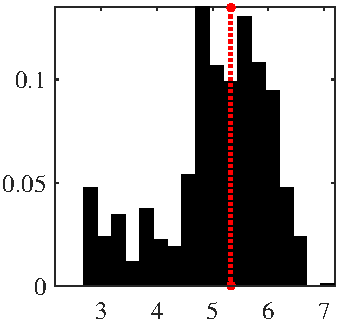
\includegraphics[scale=1]{dstats/CMD-adi-ISI.pdf}} \hspace{0.5cm} 
\subfloat[\Gls{rupaka}]{\label{fig:dstats:CMD:ISI:rupaka}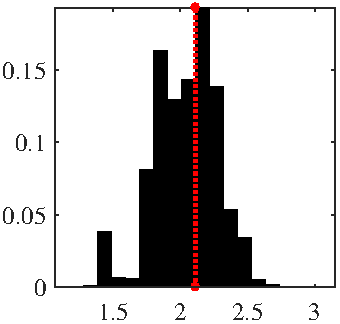
\includegraphics[scale=1]{dstats/CMD-rupaka-ISI.pdf}} \\ 
\subfloat[\Gls{mishra chapu}]{\label{fig:dstats:CMD:ISI:mishraChapu}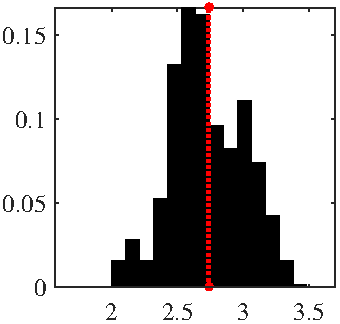
\includegraphics[scale=1]{dstats/CMD-mishraChapu-ISI.pdf}} \hspace{0.5cm} 
\subfloat[\Gls{khanda chapu}]{\label{fig:dstats:CMD:ISI:khandaChapu}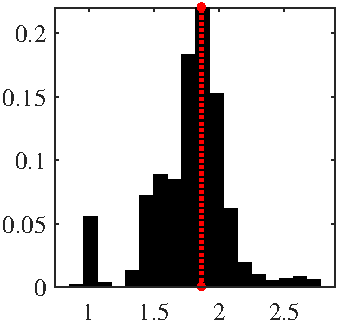
\includegraphics[scale=1]{dstats/CMD-khandaChapu-ISI.pdf}} \\ 
\caption[CMD-ISI]{CMD-ISI}\label{fig:dstats:CMD:ISI}
\end{center}
\end{figure}
%
%
% Dataset stats: CMD-ISInorm
\begin{figure}[ht]
%\captionsetup[subfigure]{labelformat=empty}
\begin{center}
\subfloat[\Gls{adi}]{\label{fig:dstats:CMD:ISInorm:adi}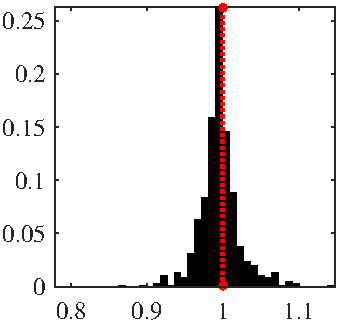
\includegraphics[scale=1]{dstats/CMD-adi-ISInorm.pdf}} \hspace{0.5cm} 
\subfloat[\Gls{rupaka}]{\label{fig:dstats:CMD:ISInorm:rupaka}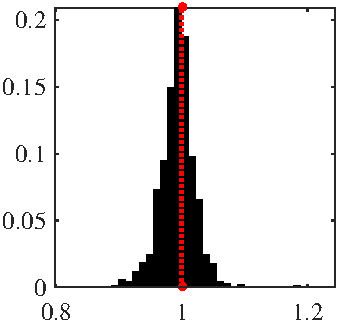
\includegraphics[scale=1]{dstats/CMD-rupaka-ISInorm.pdf}} \\ 
\subfloat[\Gls{mishra chapu}]{\label{fig:dstats:CMD:ISInorm:mishraChapu}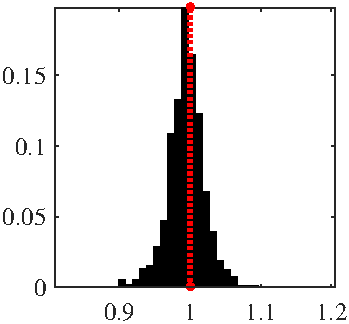
\includegraphics[scale=1]{dstats/CMD-mishraChapu-ISInorm.pdf}} \hspace{0.5cm} 
\subfloat[\Gls{khanda chapu}]{\label{fig:dstats:CMD:ISInorm:khandaChapu}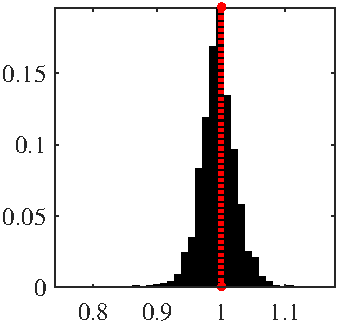
\includegraphics[scale=1]{dstats/CMD-khandaChapu-ISInorm.pdf}} \\ 
\caption[CMD-ISInorm]{CMD-ISInorm}\label{fig:dstats:CMD:ISInorm}
\end{center}
\end{figure}
%\clearpage
%% Dataset stats: CMDf-IAI
\begin{figure}[ht]
%\captionsetup[subfigure]{labelformat=empty}
\begin{center}
\subfloat[\Gls{adi}]{\label{fig:dstats:CMDf:IAI:adi}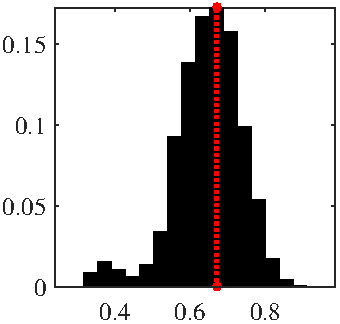
\includegraphics[scale=1]{dstats/CMDf-adi-IAI.pdf}} \hspace{0.5cm} 
\subfloat[\Gls{rupaka}]{\label{fig:dstats:CMDf:IAI:rupaka}\includegraphics[scale=1]{dstats/CMDf-rupaka-IAI.pdf}} \\ 
\subfloat[\Gls{mishra chapu}]{\label{fig:dstats:CMDf:IAI:mishraChapu}\includegraphics[scale=1]{dstats/CMDf-mishraChapu-IAI.pdf}} \hspace{0.5cm} 
\subfloat[\Gls{khanda chapu}]{\label{fig:dstats:CMDf:IAI:khandaChapu}\includegraphics[scale=1]{dstats/CMDf-khandaChapu-IAI.pdf}} \\ 
\caption[CMDf-IAI]{CMDf-IAI}\label{fig:dstats:CMDf:IAI}
\end{center}
\end{figure}
%
%
% Dataset stats: CMDf-IAInorm
\begin{figure}[ht]
%\captionsetup[subfigure]{labelformat=empty}
\begin{center}
\subfloat[\Gls{adi}]{\label{fig:dstats:CMDf:IAInorm:adi}\includegraphics[scale=1]{dstats/CMDf-adi-IAInorm.pdf}} \hspace{0.5cm} 
\subfloat[\Gls{rupaka}]{\label{fig:dstats:CMDf:IAInorm:rupaka}\includegraphics[scale=1]{dstats/CMDf-rupaka-IAInorm.pdf}} \\ 
\subfloat[\Gls{mishra chapu}]{\label{fig:dstats:CMDf:IAInorm:mishraChapu}\includegraphics[scale=1]{dstats/CMDf-mishraChapu-IAInorm.pdf}} \hspace{0.5cm} 
\subfloat[\Gls{khanda chapu}]{\label{fig:dstats:CMDf:IAInorm:khandaChapu}\includegraphics[scale=1]{dstats/CMDf-khandaChapu-IAInorm.pdf}} \\ 
\caption[CMDf-IAInorm]{CMDf-IAInorm}\label{fig:dstats:CMDf:IAInorm}
\end{center}
\end{figure}
%
%
% Dataset stats: CMDf-ISI
\begin{figure}[ht]
%\captionsetup[subfigure]{labelformat=empty}
\begin{center}
\subfloat[\Gls{adi}]{\label{fig:dstats:CMDf:ISI:adi}\includegraphics[scale=1]{dstats/CMDf-adi-ISI.pdf}} \hspace{0.5cm} 
\subfloat[\Gls{rupaka}]{\label{fig:dstats:CMDf:ISI:rupaka}\includegraphics[scale=1]{dstats/CMDf-rupaka-ISI.pdf}} \\ 
\subfloat[\Gls{mishra chapu}]{\label{fig:dstats:CMDf:ISI:mishraChapu}\includegraphics[scale=1]{dstats/CMDf-mishraChapu-ISI.pdf}} \hspace{0.5cm} 
\subfloat[\Gls{khanda chapu}]{\label{fig:dstats:CMDf:ISI:khandaChapu}\includegraphics[scale=1]{dstats/CMDf-khandaChapu-ISI.pdf}} \\ 
\caption[CMDf-ISI]{CMDf-ISI}\label{fig:dstats:CMDf:ISI}
\end{center}
\end{figure}
%
%
% Dataset stats: CMDf-ISInorm
\begin{figure}[t]
%\captionsetup[subfigure]{labelformat=empty}
\begin{center}
\subfloat[\Gls{adi}]{\label{fig:dstats:CMDf:ISInorm:adi}\includegraphics[scale=1]{dstats/CMDf-adi-ISInorm.pdf}} \hspace{0.5cm} 
\subfloat[\Gls{rupaka}]{\label{fig:dstats:CMDf:ISInorm:rupaka}\includegraphics[scale=1]{dstats/CMDf-rupaka-ISInorm.pdf}} \\ 
\subfloat[\Gls{mishra chapu}]{\label{fig:dstats:CMDf:ISInorm:mishraChapu}\includegraphics[scale=1]{dstats/CMDf-mishraChapu-ISInorm.pdf}} \hspace{0.5cm} 
\subfloat[\Gls{khanda chapu}]{\label{fig:dstats:CMDf:ISInorm:khandaChapu}\includegraphics[scale=1]{dstats/CMDf-khandaChapu-ISInorm.pdf}} \\ 
\caption[CMDf-ISInorm]{CMDf-ISInorm}\label{fig:dstats:CMDf:ISInorm}
\end{center}
\end{figure}
%
%
%%%%%%%%%%%%%%%%%